\chapter{Introduzione ai sistemi Web}
Cosa vedremo nelle prossime lezioni:
\\Applicazioni Web (lezione di oggi e giovedì)
\begin{itemize}
    \item Web come piattaforma
    \item Architettura di un'applicazione Web
\end{itemize}
Client side: HTML
\\Server side: Servlet
\begin{itemize}
    \item Il modello
    \item HTTP Servlet
\end{itemize}
Server side: JSP
\begin{itemize}
    \item Struttura di una JSP
    \item Gli elementi che compongono una JSP
    \item JSP e JavaBeans
\end{itemize}
Il pattern MVC

\section{Applicazioni Web}
\subsubsection{Perché il Web?}
Basato su Internet (non è la stessa cosa!)
\begin{itemize}
    \item Ambiente standard (alla base c'è TCP/IP)
    \item Ampia diffusione
\end{itemize}
Semplicità e uniformità dell'interazione
\begin{itemize}
    \item Interfaccia grafica (Browsers)
    \item Interazione attraverso un protocollo standard (HTTP)
    \item Definizione di una API - Application Programming Interface (applicazioni REST, vedremo meglio)
\end{itemize}
Infrastruttura completa
\begin{itemize}
    \item Supporta sistemi aperti (connessione dinamica di nuovi componenti)
    \item Strumenti sempre più completi e potenti: evoluzioni di HTML, Ajax, Web App…
\end{itemize}

\subsection{Caratteristiche principali di un'applicazione Web}
Applicazione Web = adozione del protocollo HTTP
\\Oggigiorno è essenziale avere un'infarinatura di come funzioni il protocollo HTTP.
\subsubsection{Caratteristiche del protocollo HTTP}
Formato a caratteri (lento): occorre tradurre e ritradurre i dati (es. da testo a numeri: da “256” a 256)
\\Utilizzo del linguaggio HTML per input e output:
\begin{itemize}
    \item Uso di FORM per l'acquisizione dati (invio dati al server, lato front-end)
    \item Uso di pagine HTML in risposta (dal server verso il client, lato back-end)
    \item Possibilità di pagine dinamiche (JavaScript con dati scambiati in JSON)
\end{itemize}
(A proposito di invio di dati, ci sono due modi: appunto i FORM, ma anche le QUERIES.)
\\Utilizzo di payload di tipo MIME (Multimedia Internet Mail Extensions)
\begin{itemize}
    \item Permettono di generalizzare oltre HTML (xml, json, zip, jpeg)
    \item 
\end{itemize}
Conversazioni (interazioni client-server) prive di stato (memoria)
\begin{itemize}
    \item Ogni richiesta è un messaggio autonomo, indipendente dagli altri.
    \item Per creare sessioni di lavoro (legare più richieste tra loro) servono informazioni esplicite (cookies, campi nascosti).
    \item Un cookie HTTP (web cookie, browser cookie) è un piccolo blocco di dati che un server invia al browser web di un utente. Il browser può memorizzare il cookie e rinviarlo allo stesso server con richieste successive. In genere, un cookie viene utilizzato per stabilire se due richieste provengono dallo stesso browser, ad esempio per mantenere un utente loggato.
    \item \`E impossibile pensare di creare un applicativo privo di stato, pensiamo solo alla sessione di attività dell'utente.
\end{itemize}

\subsection{Dal Web alle Applicazioni Web}
Il Web supporta l'interazione tra client e server via HTTP
\\Ben presto il web si è evoluto andando al di là del trasferimento di pagine web (file HTML). \`E diventato uno strumento per fornire accesso ad applicazioni remote
\\Per eseguire una applicazione, il Web Server utilizza un Application Server
\\Un Application server è caratterizzato dal protocollo di interazione con il Web Server
\\L'interazione con il client avviane sempre tramite HTTP 
\begin{center}
    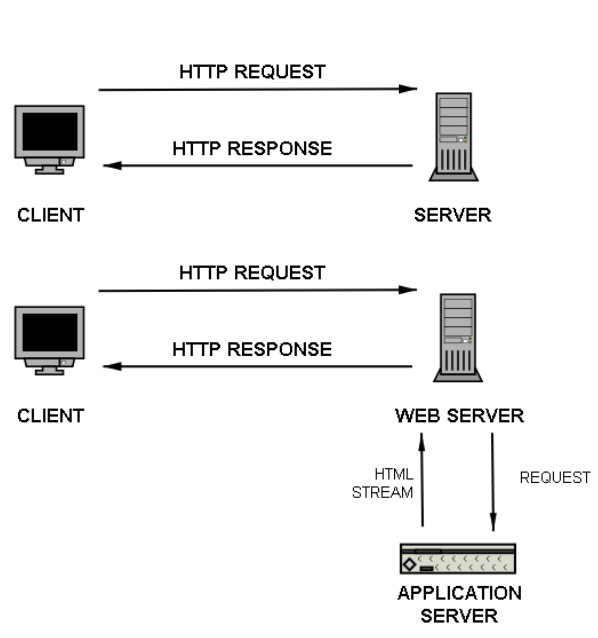
\includegraphics[width=0.675\textwidth]{img/appWeb1.jpg}
\end{center}

\subsubsection{Tecnologia Server Side}
La computazione avviene lato server e può avvenire tramite \textbf{\textit{programmi (compilati)}} o \textbf{\textit{script (interpretati)}}.
\\Nel caso di programmi compilati il Web Server si limita ad invocare, su richiesta del client, un eseguibile.
\begin{itemize}
    \item L'eseguibile può essere scritto in un qualsiasi linguaggio che supporti l'interazione con il Web Server
    \item Tra i linguaggi più diffusi C\#, C++.
\end{itemize}
Nel caso di esecuzione di script, il Web Server ha al suo interno un motore (engine) in grado di interpretare il linguaggio di scripting usato.
\begin{itemize}
    \item Si perde in velocità di esecuzione (parliamo di latenza, più che di velocità), ma si guadagna in facilità di scrittura dei programmi.
    \item Tra i linguaggi più diffusi Java, PHP, Pyton e Perl, più recentemente Nodejs.
\end{itemize}
\begin{center}
    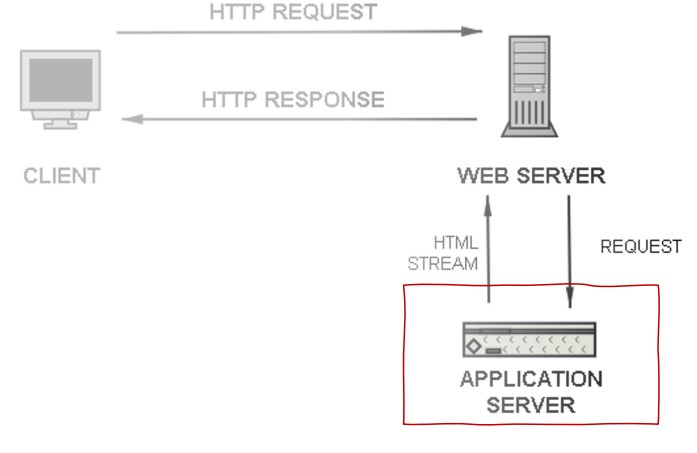
\includegraphics[width=0.675\textwidth]{img/appWeb2.jpg}
\end{center}

\subsubsection{Architettura di un'applicazione compilata}
Uniform Resource Locator (URL)
\begin{itemize}
    \item definisce un naming globale
\end{itemize}
HyperText Transfer Protocol (HTTP)
\begin{itemize}
    \item permette di invocare i programmi sul server come fossero risorse
\end{itemize}
Questa parte è valida anche per applicazioni interpretate.
\\Common Gateway Interface (CGI). Protocollo che permette al server di:
\begin{itemize}
    \item attivare un programma (crea un processo)
    \item passargli le richieste e i parametri provenienti dal client 
    \item recuperare la risposta
\end{itemize}
Ogni applicazione CGI deve quindi implementare l'interprete del protocollo.
\begin{center}
    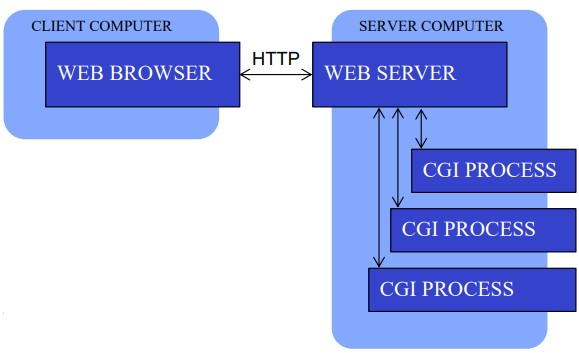
\includegraphics[width=0.675\textwidth]{img/appWeb3.jpg}
\end{center}
Quando un client richiede al server un URL corrispondente a un documento HTML, il server restituisce il documento stesso come un file di testo. Ciò significa che il documento viene generato una volta per tutte e poi viene inviato al client senza ulteriori elaborazioni. Quando l'URL richiesto corrisponde a un'applicazione CGI, il server esegue il programma in tempo reale, generando dinamicamente informazioni per l'utente. 

\subsubsection{Architettura di un'applicazione interpretata}
Il protocollo CGI viene gestito dall'interprete per il linguaggio usato (le applicazioni NON devono più gestire il protocollo CGI).
\\\textbf{Vantaggi:}
\begin{itemize}
    \item Serve programmare solo le logiche delle applicazioni
    \item Modello delle applicazioni conformi al modello del linguaggio utilizzato
    \item Semplicità, portabilità, manutenibilità
\end{itemize}
Esempi
\begin{itemize}
    \item Python
    \item Java/Servlet
    \item PHP
    \item Nodejs
\end{itemize}
\begin{center}
    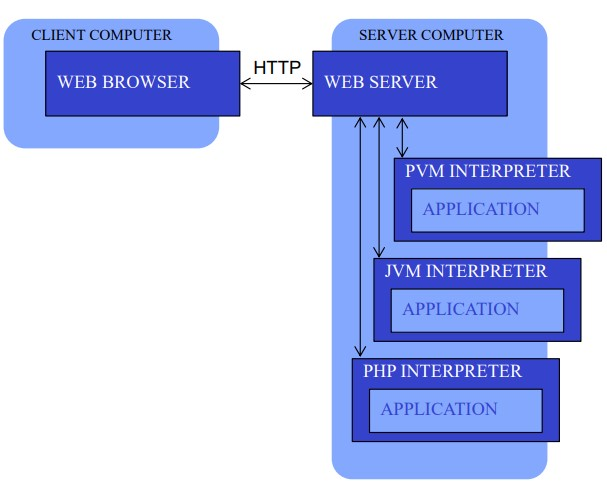
\includegraphics[width=0.675\textwidth]{img/appWeb4.jpg}
\end{center}

\section{Client Side - HTML}
\subsection{Richieste}
\subsubsection{Basate su Link}
Un link in un documento HTML può essere usato per puntare ad una risorsa remota:
\begin{verbatim}
    <p>Click the link to ask the servlet to send back an HTML document</p>
    <a href="http://localhost:8080/SlideServlet/GetHTTPServlet">
        Get HTML Document
    </a>
\end{verbatim}
Il browser invia richieste del tipo:
\begin{verbatim}
    GET /SlideServlet/GetHTTPServlet HTTP/1.1
\end{verbatim}

\subsubsection{Per mezzo di FORM}
Anche il parametro action di un Form può essere usato per puntare ad una risorsa remota (applicazione)
\begin{verbatim}
    <form action="http://localhost:8080/SlideServlet/GetHTTPServlet" method="GET">
        <p>Click the button to have the servlet send an HTML document</p>
        <input type="submit" value="Get HTML Document">
    </form>
\end{verbatim}
Il browser invia richieste del tipo:
\begin{verbatim}
    GET /SlideServlet/GetHTTPServlet HTTP/1.1
\end{verbatim}

% Mi sono persa un sacco di slides, quelle col codice arancino screenshottale così come sono. Il resto copia e incolla, che è tutto codice.

\section{Server Side - Java Servlet}
\subsection{Java Servlets}
Estensione della classe Servlet che risiede su un application server che la può gestire.

\subsubsection{Ma cosa sono?}
Sono piccole applicazioni Java residenti sul server (esempio: Apache Tomcat).
\\Una servlet è un componente gestito in modo automatico da un container o engine.
\\Deve implementare un'interfaccia prestabilita che definisce il set di metodi:
\begin{itemize}
    \item \textbf{Vantaggi:} semplicità e standardizzazione
    \item \textbf{Svantaggi:} rigidità del modello
\end{itemize}
Il container controlla le servlet (le attiva/disattiva) in base alle richieste dei client. Questo è possibile in
maniera automatica perché le servlet implementano una interfaccia nota al server.
\\Sono oggetti Java residenti in memoria, quindi
\begin{itemize}
    \item mantengono uno stato
    \item consentono l'interazione con altre servlet
\end{itemize}

\subsubsection{Stateless vs. stateful}
HTTP non prevede persistenza (\textit{stateless}).
\begin{itemize}
    \item Non si possono mantenere informazioni tra un messaggio e i successivi.
    \item Non si possono identificare i client.
\end{itemize}
Mantenere lo stato della conversazione è compito dell'applicazione (se vuole). Gli strumenti:
\begin{description}
    \item[Cookies:] 
    \\- Informazioni memorizzate a livello di client;
    \\- Permettono di gestire sessioni di lavoro.
    \item[HTTPSession:] 
    \\- Oggetto gestito automaticamente dal container/engine (con cookie o riscrittura delle URL);
    \\- Le servlet possono accedervi per immagazzinare informazioni.
    \\Da considerare come una mappa chiave-valore.
\end{description}
Ovviamente i dati possono essere memorizzati anche in un database. Quale sarebbe il vantaggio di un HTTPSession invece di un Database?
\\\`E uno strumento già pronto, poi le informazioni lì immagazzinate sono \textbf{volatili} e in alcune situazioni torna utile.
\\Es.: prenotazione del biglietto di un treno. Se l'utente (per cui il biglietto in fase di acquisto è prenotato tra il momento della scelta del biglietto e quello dell'acquisto) non compra in diciamo 15 minuti, l'informazione dell'acquisto è persa e il biglietto torna disponibile per la vendita per altri clienti.
\\Es.: invece il carrello di Amazon non lo è, volatile. Amazon si ricorda della scelta dell'utente e gli ripropone l'articolo anche in tempi futuri.

\subsection{Interfaccia Servlet}
Ogni servlet implementa l'interfaccia jakarta.servlet.Servlet, con 5 metodi
\begin{verbatim}
    void init(ServletConfig config)
\end{verbatim}
Inizializza la servlet, viene invocato dopo la creazione della stessa
\begin{verbatim}
    void destroy()
\end{verbatim}
Chiamata quando la servlet termina (es: per chiudere un file o una connessione con un database)
\begin{verbatim}
    void service(ServletRequest request, ServletResponse response)
\end{verbatim}
Invocato per gestire le richieste dei client
\begin{verbatim}
    ServletConfig getServletConfig()
\end{verbatim}
Restituisce i parametri di inizializzazione e il ServletContext che da accesso all'ambiente
\begin{verbatim}
    String getServletInfo()
\end{verbatim}
Restituisce informazioni tipo autore e versione

\subsection{Classi astratte}
L'interfaccia è solo la dichiarazione dei metodi che, per essere utilizzabili, devono essere implementati in una classe.
\\Sono presenti due classi astratte, cioè che implementano i metodi dell'interfaccia in modo che non facciano nulla.
\begin{verbatim}
    jakarta.servlet.GenericServlet
\end{verbatim}
Definisce metodi indipendenti dal protocollo
\begin{verbatim}
    jakarta.servlet.http.HTTPServlet
\end{verbatim}
Definisce metodi per l'uso in ambiente web.
\\Questo semplifica l'implementazione delle servlet vere e proprie in quando basta implementare (ridefinendoli) solo i metodi che interessano.

\subsection{La classe HTTPServlet}
Implementa service() in modo da invocare i metodi per servire le richieste dal web.
\begin{description}
    \item[Metodi doX] 
    \\ X è un metodo HTTP (doGet, doPost, …)
    \\ doX è dedicato alle richieste di tipo X
    \item[Parametri:]
    \\ HTTPServletRequest
    \\ HTTPServletResponse
    \item[Eccezioni]
    \\ ServletException
    \\ IOException
\end{description}
\begin{center}
    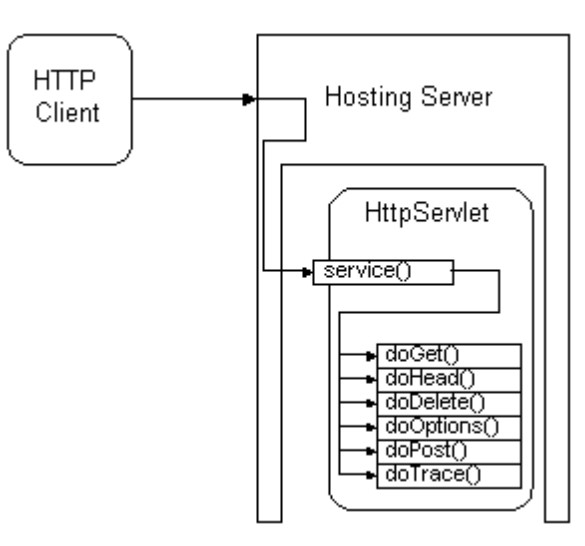
\includegraphics[width=0.5\textwidth]{img/appWeb7.jpg}
\end{center}

\subsection{Richieste e risposte}
Anche i parametri sono stati adattati al protocollo HTTP, cioè consentono di ricevere (inviare) messaggi HTTP leggendo (scrivendo) i dati nell'header e nel body di un messaggio.
\\Interfaccia HTTPServletRequest
\begin{itemize}
    \item Viene passato un oggetto da service
    \item Contiene la richiesta del client
    \item Estende ServletRequest
\end{itemize}
Interfaccia HTTPServletResponse
\begin{itemize}
    \item Viene passato un oggetto da service
    \item Contiene la risposta destinata al client
    \item Estende ServletResponse
\end{itemize}

I metodi principali per le \textbf{richieste}:
\begin{description}
    \item[String getParameter(String name)] - Restituisce il valore del query parameter dato il nome (valore singolo)
    \item[Enumeration getParameterNames()] - Restituisce l'elenco dei nomi degli argomenti
    \item[String[] getParametersValues(String name)] - Restituisce i valori dell'argomento name (valore multiplo)
\end{description}

I metodi principali per le \textbf{risposte}:
\begin{description}
    \item[void setContentType(String type)] - Specifica il tipo MIME della risposta per dire al browser come
    visualizzare la risposta Es: “text/html” dice che è html
    \item[ServletOutputStream getOutputStream()] - Restituisce lo stream di byte per scrivere la risposta
    \item[PrintWriter getWriter()] - Restituisce lo stream di caratteri per scrivere la risposta
\end{description}

Altri metodi
\begin{description}
    \item[Cookie[] getCockies()] - Restituisce i cookies del server sul client
    \item[void addCookie(Cookie cookie)] - Aggiunge un cookie nell'intestazione (header) della risposta
    \item[HTTPSession getSession(boolean create)] - Una HTTPSession dentifica il client.
    \\Viene creata se create=true
\end{description}
